%This is the first chapter of the dissertation

%The following command starts your chapter. If you want different titles used in your ToC and at the top of the page throughout the chapter, you can specify those values here. Since Columbia doesn't want extra information in the headers and footers, the "Top of Page Title" value won't actually appear.

\chapter[Recursive Jigsaw Reconstruction][Recursive Jigsaw Reconstruction]{Recursive Jigsaw Reconstruction}
\label{ch:jigsaw}

\textit{Recursive Jigsaw Reconstruction} (RJR) ~\cite{Jackson:2016mfb,ATLAS-CONF-2016-078} is a novel algorithm used for the analysis presented in this thesis.
RJR is the conceptual successor to the razor technique ~\cite{Rogan:2010kb,Buckley:2013kua}, which has been used successfully in many new physics searches ~\cite{SUSY-2014-05,SUSY-2014-06,CMS-SUS-13-004,CMS-SUS-12-005,CMS-SUS-11-024,SUSY-2011-22}.
In this chapter, we will first present the razor technique, and describe the razor variables.
We will then present the RJR algorithm.
After the description of the algorithm, we will describe the precise RJR variables used in the analysis.

\section{Razor variables}

\subsection{Motivation}
We consider SUSY models where gluinos and squarks are pair-produced.
Pair-production is a consequence of the $R$-parity imposed in many SUSY models.
$R$-parity violation is highly constrained by limits on proton decay~\cite{susyPrimer}, and is often assumed in SUSY model building.
The Feynman diagrams considered are shown in \Cref{fig:feynman_signal}.
\begin{figure}[tbp]
\caption{Feynman diagrams for the SUSY signals considered in this thesis} \label{fig:feynman_signal}
\subfloat[Squark pair production]   {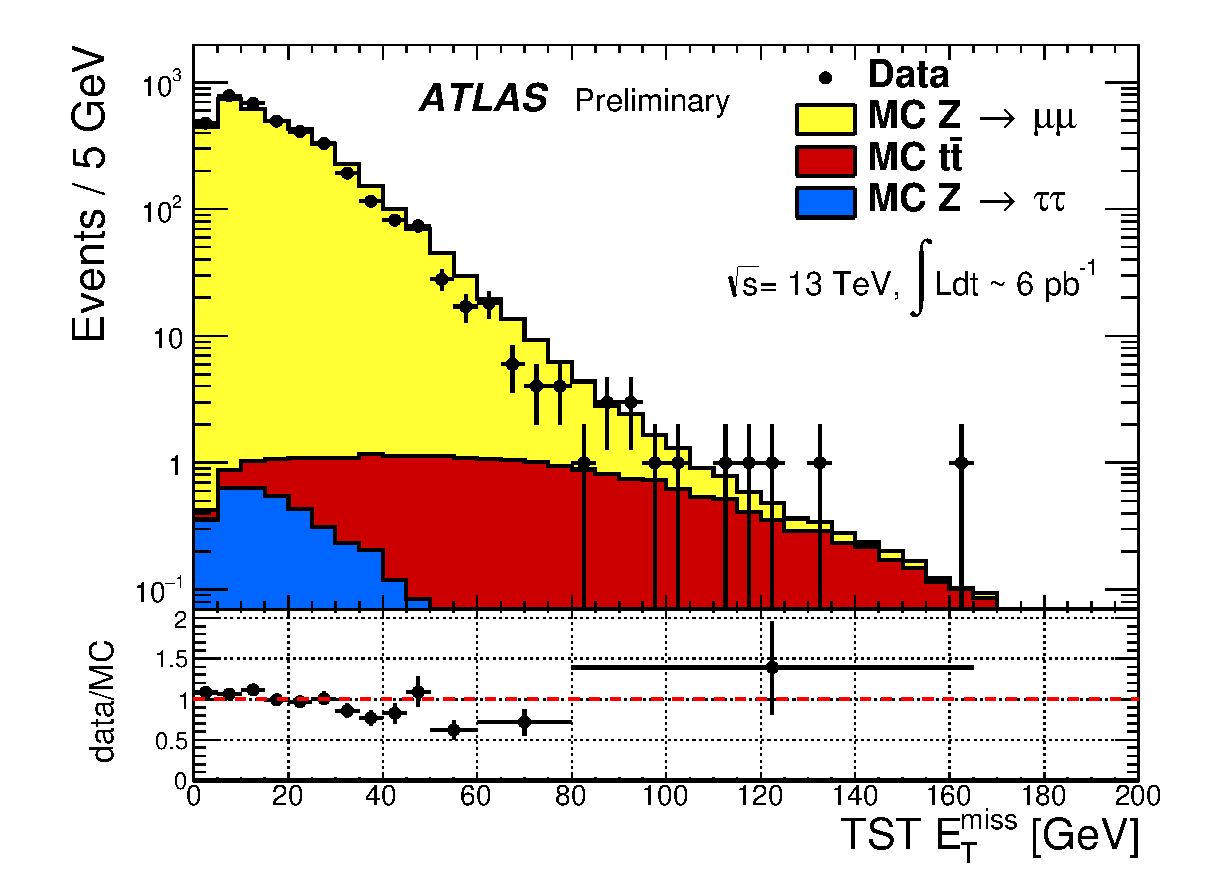
\includegraphics[width=.7\linewidth]{ATLAS-CONF-2016-078/fig_01a}} \\
\subfloat[Gluino pair production]   {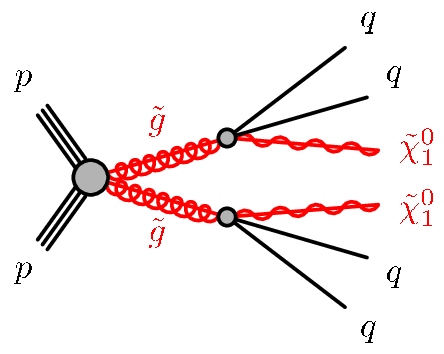
\includegraphics[width=.7\linewidth]{ATLAS-CONF-2016-078/fig_01b}} \\
\end{figure}

The consequences of this $\mathbb{Z}_2$ symmetry are drastic~\cite{susyPrimer}.
To understand the utility of the razor variables, the stability of the lightest supersymmetric particle is important.
In many SUSY models, including the ones considered in this thesis, this is the lightest neutralino \lsp.
This means that on either side of a SUSY decay process, where we begin with sparticle pair production, we have a final state particle which is not detected.
Generically, this leads to \met.
Selections based on \met are very good at reducing  backgrounds, for example from QCD processes.

However, there are limitations to searches based on \met.
Due to jet mismeasurements, instrumental failures, finite detector acceptance, nongaussian tails in the detector response, and production of neutrinos inside of jets, there are many sources of ``fake'' \met which does not correspond to a Standard Model neutrino or new physics object such as an LSP.
An additional limitation is the complete lack of longitudinal information.
As events from QCD backgrounds tend to have higher boosts along the $z$-direction, this neglects an important discriminator for use in searches for SUSY.
Finally, \met is only one object, which is a measurement for \textit{two} separate LSPs.
If one could factorize this information somehow, this would provide additional information to potentially discriminate against backgrounds.
The \textit{razor variables} $(\mdr, R^2)$ are more robust than \met-based variables against sources of fake \met as well as providing additional longitudinal information which can be used to discriminate against backgrounds~\cite{Rogan:2010kb,Buckley:2013kua}.

\subsection{Derivation of the razor variables}

To derive the razor variables $(\mdr, R^2)$, we start with a generic situation of the pair production of heavy sparticles with mass $\mheavy$.\footnotemark
\footnotetext{The razor variables have undergone confusing notational changes over the years.
We will be self-consistent, but the notation used here may be different from references.
}
Each sparticle decays to a number of observable objects (in this thesis, jets), and an unobservable \lsp~ of mass \mlsp.
We will combine all of the jets into a \textit{megajet}; this process will be described below.
We begin by analyzing the decay in the ``rough-approximation'', or in modern parlance, \textit{razor frame} (\rframe).
This is the frame where the sparticle is at rest.
Note that by construction, there are two razor frames corresponding to each sparticle.
The complete set of frames considered in the case of the razor variables is shown in \Cref{fig:razor_frames}.
\begin{figure}[tbp]
\caption{Frames considered when applying the razor technique, from ~\cite{Buckley:2013kua}.} \label{fig:razor_frames}
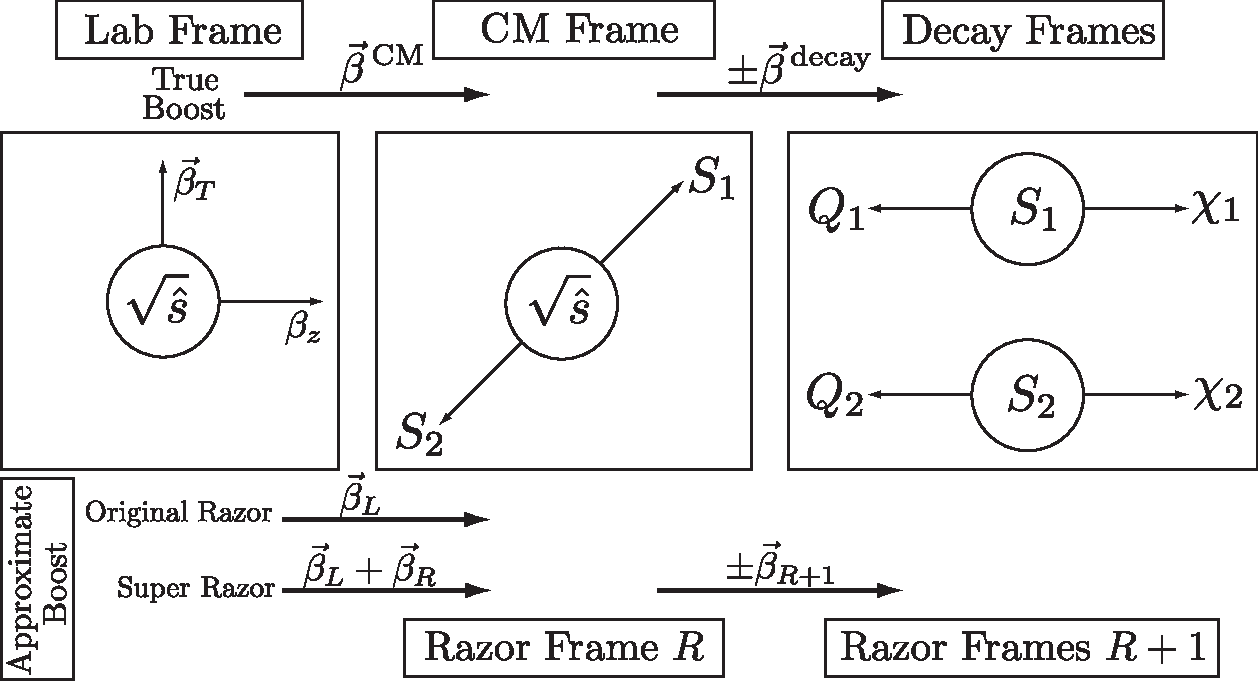
\includegraphics[width=.9\linewidth]{superrazor/fig/sectionII/frames2}
\end{figure}

In the \rframe, the decay is straightforward to analyze.
Each megajet has energy $E_1^R, E_2^R$ in the frame of its parent sparticle, and we define a characteristic mass $M_R$:
\begin{align}\label{eq:mr}
E_1^R &= E_2^R &= \frac{\mheavy^2 - \mlsp^2}{ 2 \mheavy } \\
M_R &= 2 \times E_1^R = 2 \times E_2^R &= \frac{\mheavy^2 - \mlsp^2}{\mheavy }.
\end{align}
For cases where $\mheavy >> \mlsp$, $M_R$ is an estimator of \mheavy.
This scenario happens in the SM, such as in \ttbar and \WW events, where the \lsp~ is instead a neutrino.

The question now is how to use this simple derivation in the lab frame, where we actually conduct our measurements.
There are two related issues: how to combine the jets into the megajets, and how to ``transform'' (or \textit{boost}) to the \rframe.

To construct the megajets, the procedure is the following.
For a given set of jets $j_i, i = 0 , ... , n_{\mathrm{jet}}$, we construct \textit{all} combinations of their four-momenta such that there is at least one jet inside each megajet.
Among this set of possible megajets $\{J_{1,2}\}$, we make the following unique choice for the megajets.
We minimize the following quantity:
\begin{align}
m_{J_1}^2 + m_{J_2}^2.
\end{align}
In modern parlance, this is known as a \textit{jigsaw}.
This is a \textit{choice}.
It may have nice physical qualities or satisfy some convenient intuition about the events, but as we will see later, other choices are possible.

We now describe how we translate our megajet kinematics, measured in the lab frame, to the \rframe.
This is a two-step procedure.
We perform two \textit{boosts}: a longitudinal boost $\beta_L$ and a transverse boost $\beta_T$.
Schematically,
\begin{align}
J_1^R & \xrightarrow[]{\beta_T } J_1^{CM} & \xrightarrow[]{\beta_L} J_1^{\text{lab}} \\
J_2^R & \xrightarrow[]{-\beta_T} J_2^{CM} & \xrightarrow[]{\beta_L} J_2^{\text{lab}} \\
\end{align}
The $J_{1,2}^{\text{lab}}$ correspond directly to those in the megajet construction.
We drop the ``$\text{lab}$'' designation for the rest of the discussion.
The question is how to compute the magnitudes of these boosts, given the missing degrees of freedom.

For the transverse boost $\beta_T$, recall the two megajets have equal energies in their \rframe~by construction.
This constraint can be reexpressed as a constraint on the magnitude of this boost, in terms of the boost velocity $\beta_L$ and corresponding Lorentz factor $\gamma_L$):
\begin{align}\label{eq:beta_t}
\beta_T = \frac{ \gamma_L (E_1 - E_2) - \gamma_L \beta_L (p_{1,z} - p_{2,z})}
               { \hat{\beta}_T \cdot (\vec{p_{1,T}} + \vec{p_{2,T}} )}
\end{align}
where we have denoted the lab frame four-vectors as  $p_i = (E_i , \vec{p_{i,T}} , p_z)$.
We now make the \textit{choice} for the direction of the transverse boost $\hat{\beta}_T$:
\begin{align}
\hat{\beta}_T =  \frac{\vec{p_{1,T}} +  \vec{p_{2,T}}}{ | \vec{p_{1,T}} +  \vec{p_{2,T}}  | }.
\end{align}
This choice forces the denominator of \Cref{eq:beta_t} to unity, and corresponds to aligning the transverse boost direction with the sum of the two megajets transverse directions.

For the longitudinal boost, we choose $\vec{\beta_L}$ along the $z$-direction, with magnitude:
\begin{align} \label{eq:beta_l}
\beta_L = \frac{p_{1,z} + p_{2,z}}{E_1+E_2}.
\end{align}
Viewed in terms of the original parton-parton interactions, this is the choice which ``on average'' gives $p_{z,\text{CM}} = 0$, as we would expect.
This well-motivated choice due to the total $z$ symmetry.

We now have intuitive guesses for both boosts, which allow us write our original characteristic mass $M_R$ in terms of the lab frame variables, by application of these two Lorentz boosts to the energies of \Cref{eq:mr}:
\begin{align}
M_R^2 &\xrightarrow[]{\beta_T } M_{R,\text{CM}}^{2} \xrightarrow[]{\beta_L } M_{R,\text{lab}}^{2}
      &=(E_1 + E_2)^2 - (p_{1,z} + p_{1,z})^2.
\end{align}

Finally, we define an additional mass variable, which include the missing transverse energy \met.
Importantly, note that we did not use the \met in the definition of $M_R$, which depends only on the energies of the megajets.
Backgrounds with no invisible particles (such as multijet events) must have $J_1$ and $J_2$ back to back.
Thus, we define the transverse mass:
\begin{align}
(M_R^T)^2 = \frac{1}{2} \begin{bmatrix} \met(p_{1,T}  + p_{2,T}) - \metvec \cdot (\vec{p_{1,T}}  + \vec{p_{2,T} })  \end{bmatrix}.
\end{align}
Generally, we have $M_R^T < M_R$, so we define a dimensionless ratio (``the razor''):
\begin{align}
R^2 = \begin{pmatrix} \frac{M_R^T}{M_R} \end{pmatrix}^2.
\end{align}
For signal events, we expect $R$ to peak around $R \order 1/4$, while backgrounds without real \met are expected to have $R \order 0$.

\section{Recursive Jigsaw Reconstruction}

Recursive Jigsaw Reconstruction is an algorithm allowing the imposition of a decay tree interpretation of a particular event~\cite{Jackson:2016mfb,ATLAS-CONF-2016-078}.
The idea is to construct the underlying kinematic variables (the masses and decay angles) on an event-by-event level.
This is done ``recursively'' through a decay tree which corresponds, sometimes approximately, to the Feynman diagram for the signal process of interest.
After each step of the recursive procedure, the objects are ``placed'' into one bucket (or branch) of the decay tree, and the process is repeated on each frame we have imposed.
The imposition of these decay trees is done by a \textit{jigsaw} rule: a procedure to resolve combinatoric or kinematic ambiguities while traversing the decay tree.
This procedure is performed by the \texttt{RestFrames} software packages ~\cite{RestFrames}

In events where all objects are fully reconstructed, this is straightforward, and of course has been used for many years in particle physics experiments.
Events which contain \met are more difficult, due to the loss of information: the potential for multiple mismeasured or simply unmeasureable objects, such as neutrinos or the LSP in SUSY searches.
There can also be combinatoric ambiguities in deciding how to group objects of the same type.
Specifically here, we will be concerned with the jigsaw rule to associate jets to a particular branch of a decay tree.
The jigsaw rules we impose will remove these ambiguities.
First, we will describe the decay trees used in this thesis, and then describe the jigsaw rules we will use.
Finally, we will describe the variables used in the all-hadronic SUSY search presented in this thesis.

\subsection{Decay Trees}

The decay trees imposed in this thesis are shown in \Cref{fig:decay_trees}.
\begin{figure}[tbp]
\caption{RJR decay trees} \label{fig:decay_trees}
\subfloat[Squark pair decay tree]        {\label{subfig:disquark_decay_tree}       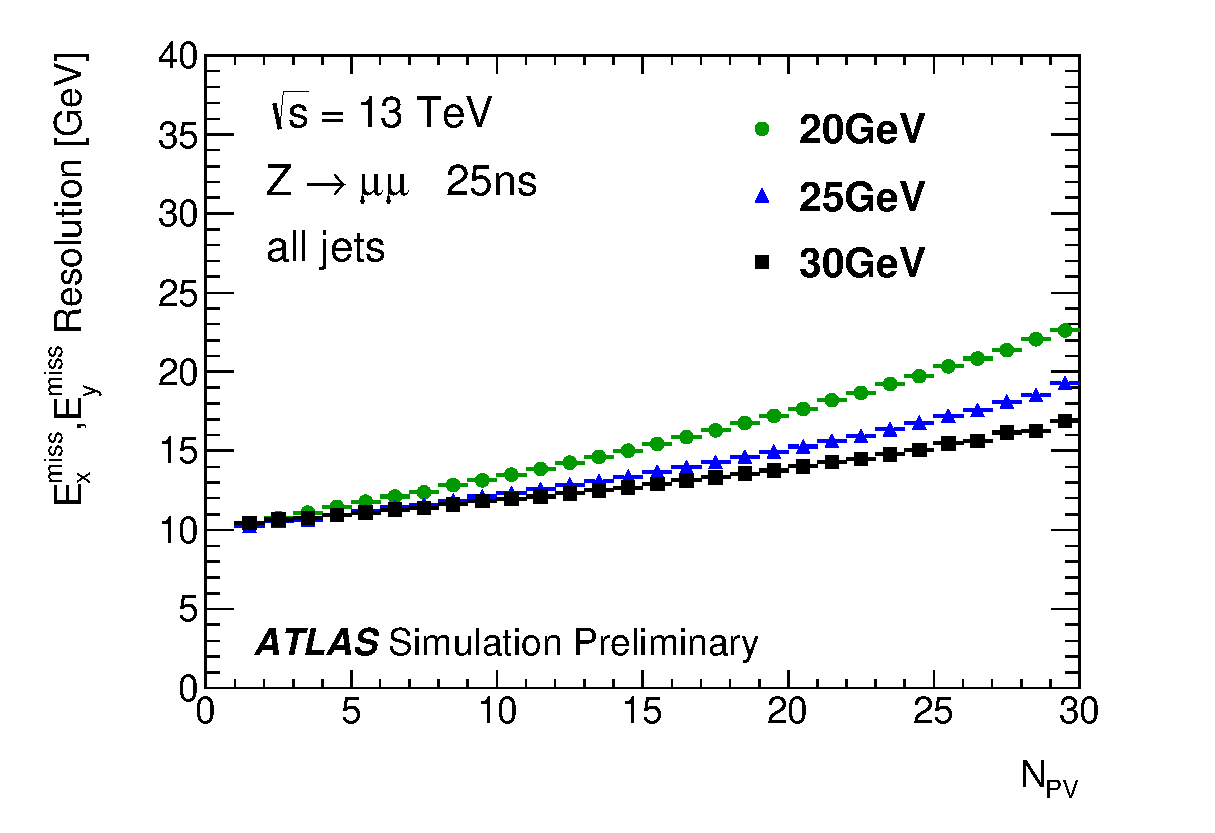
\includegraphics[width=.45\linewidth]{ATLAS-CONF-2016-078/fig_02a}}
\subfloat[Gluino pair decay tree]        {\label{subfig:digluino_decay_tree}       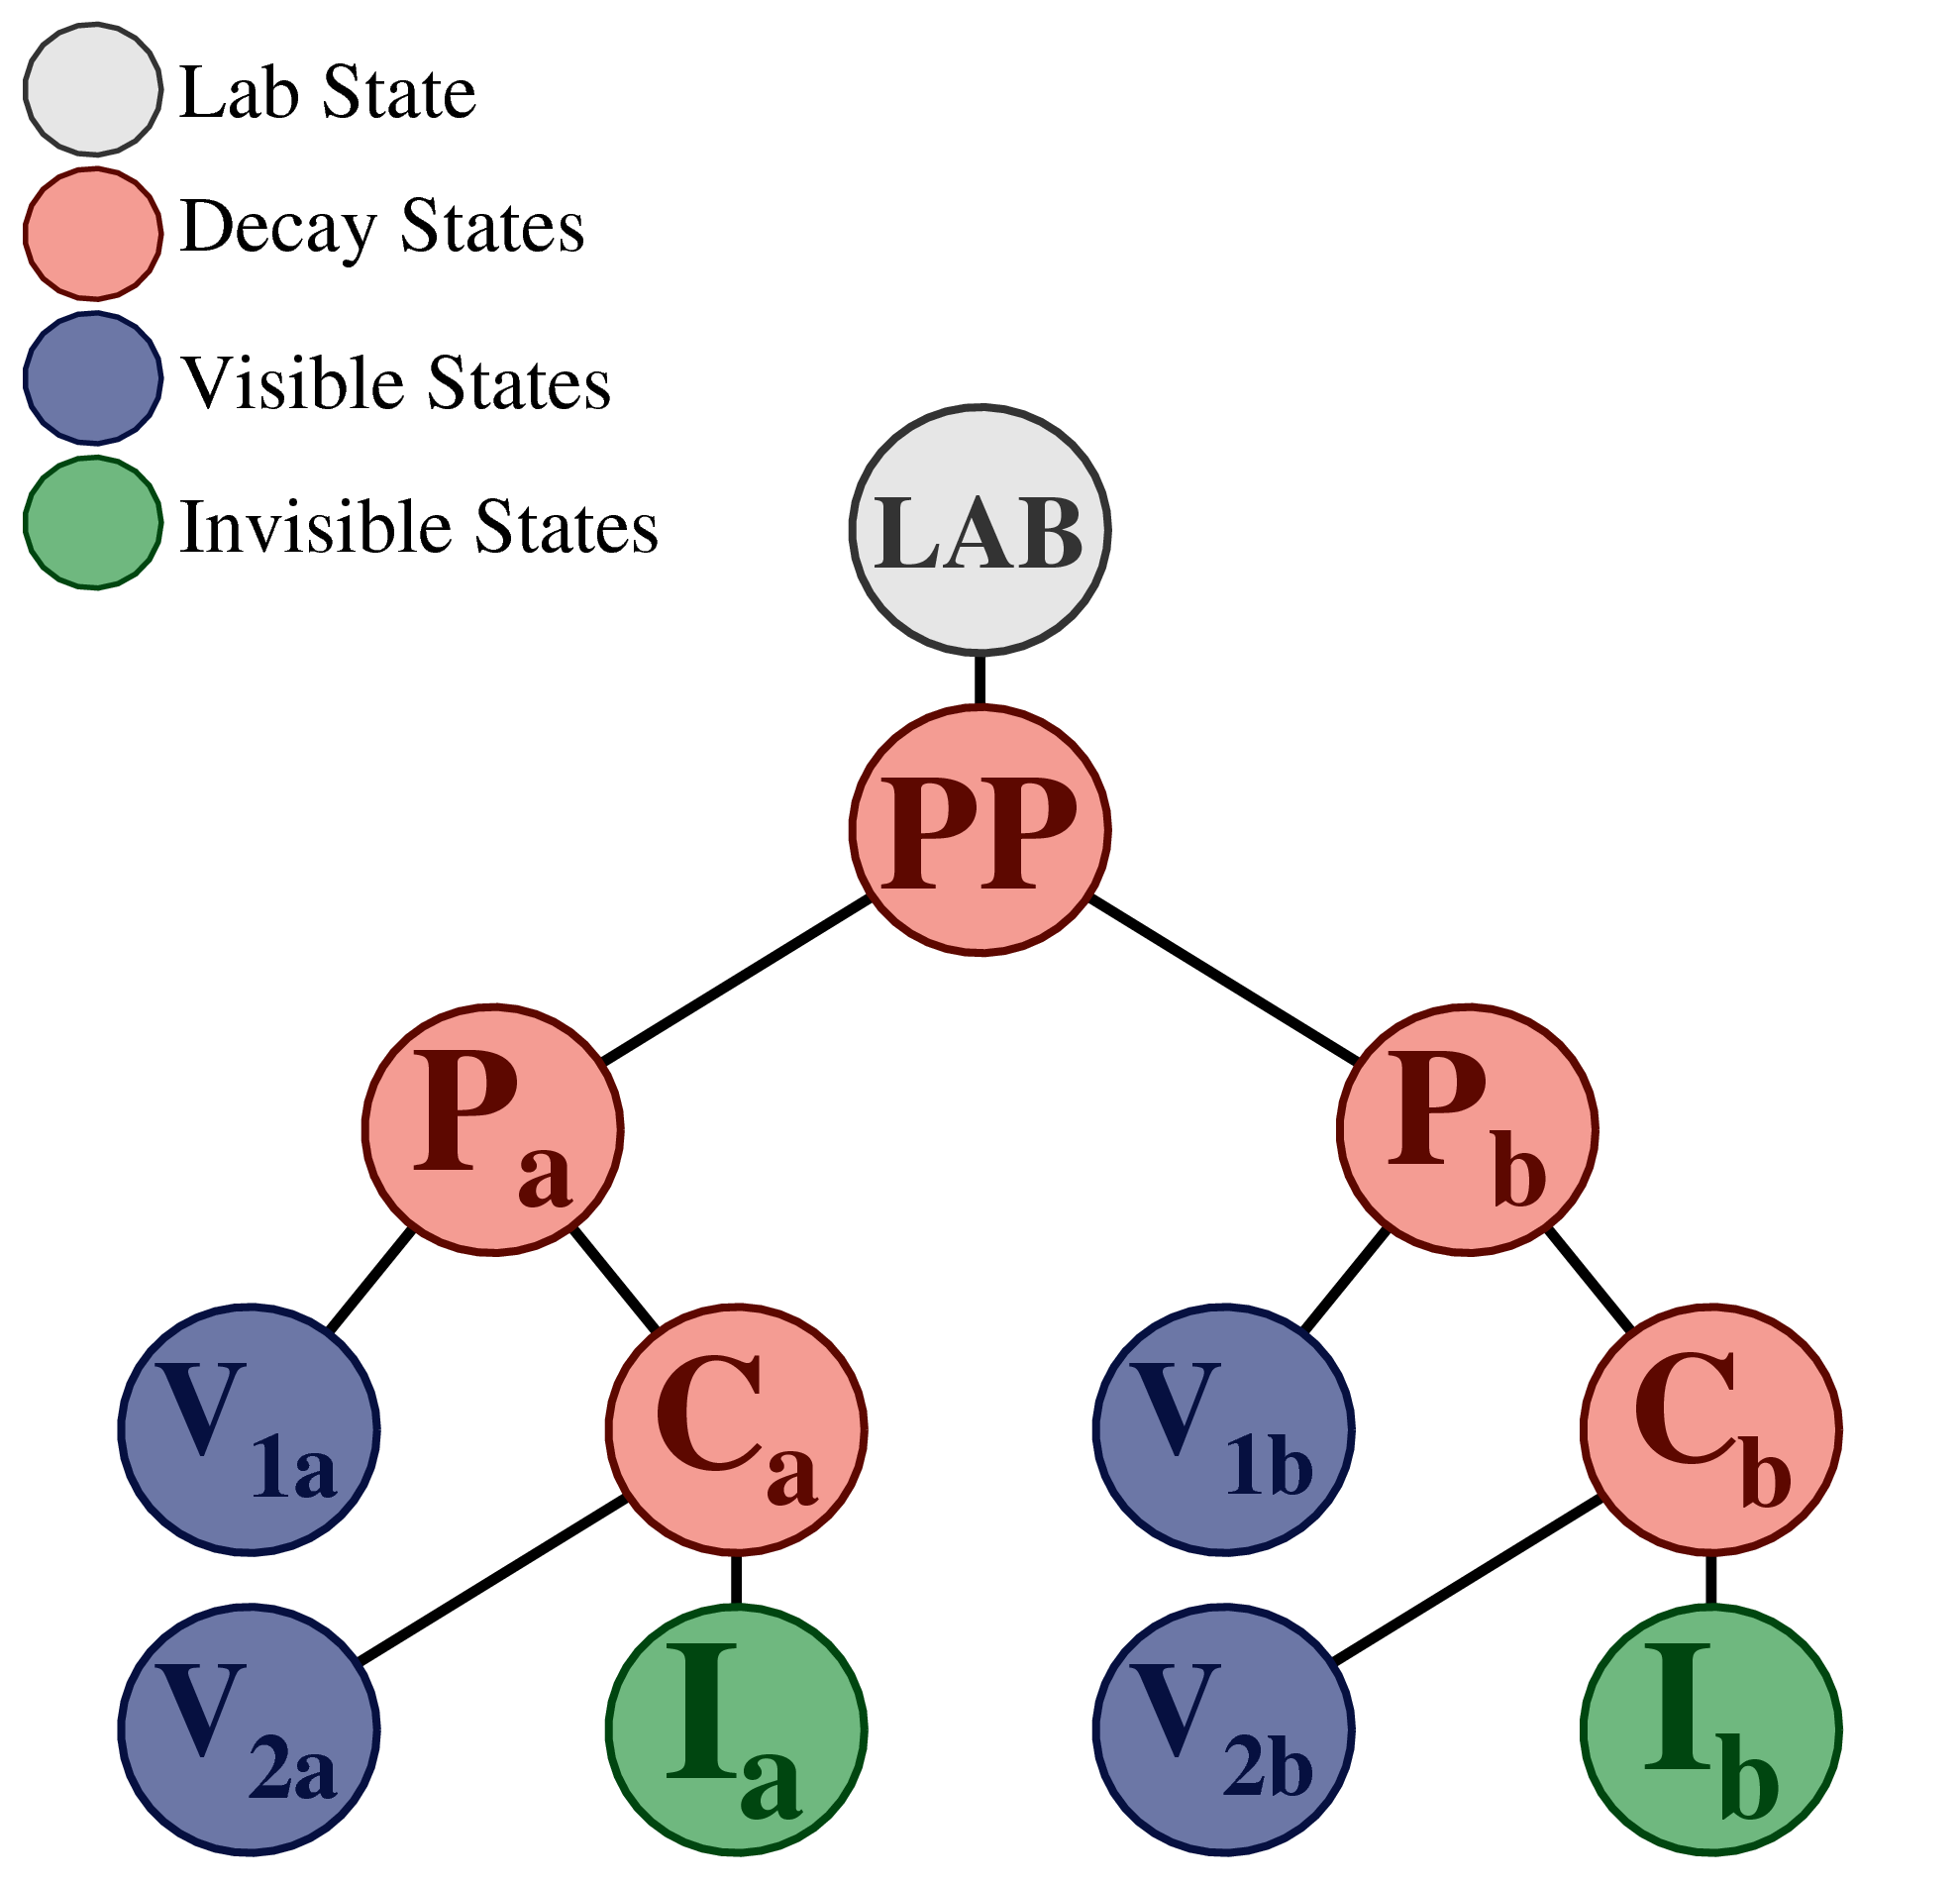
\includegraphics[width=.45\linewidth]{ATLAS-CONF-2016-078/fig_02b}} \\
\subfloat[Compressed decay tree]         {\label{subfig:compressed_decay_tree}     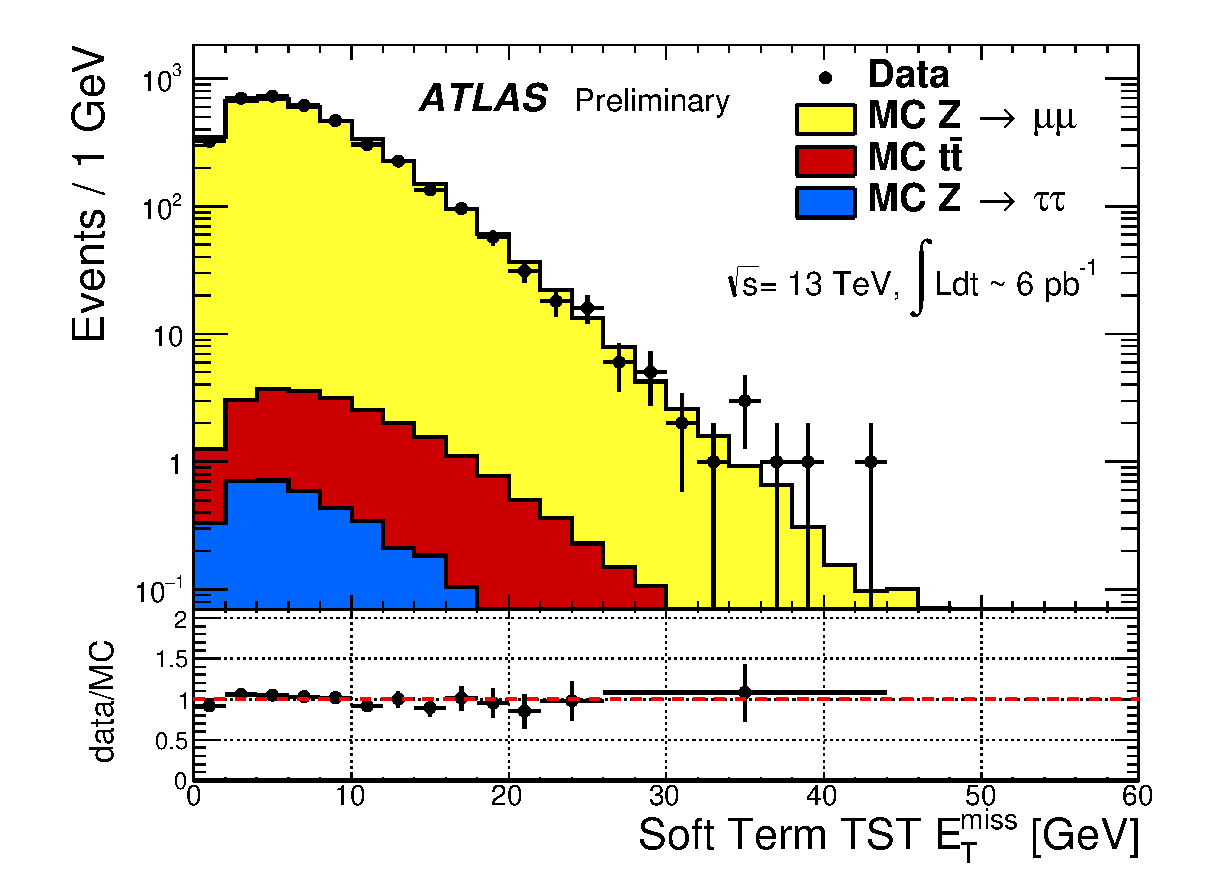
\includegraphics[width=.45\linewidth]{ATLAS-CONF-2016-078/fig_02c}}
\subfloat[Anti-QCD assembling decay tree]{\label{subfig:self_assembling_decay_tree}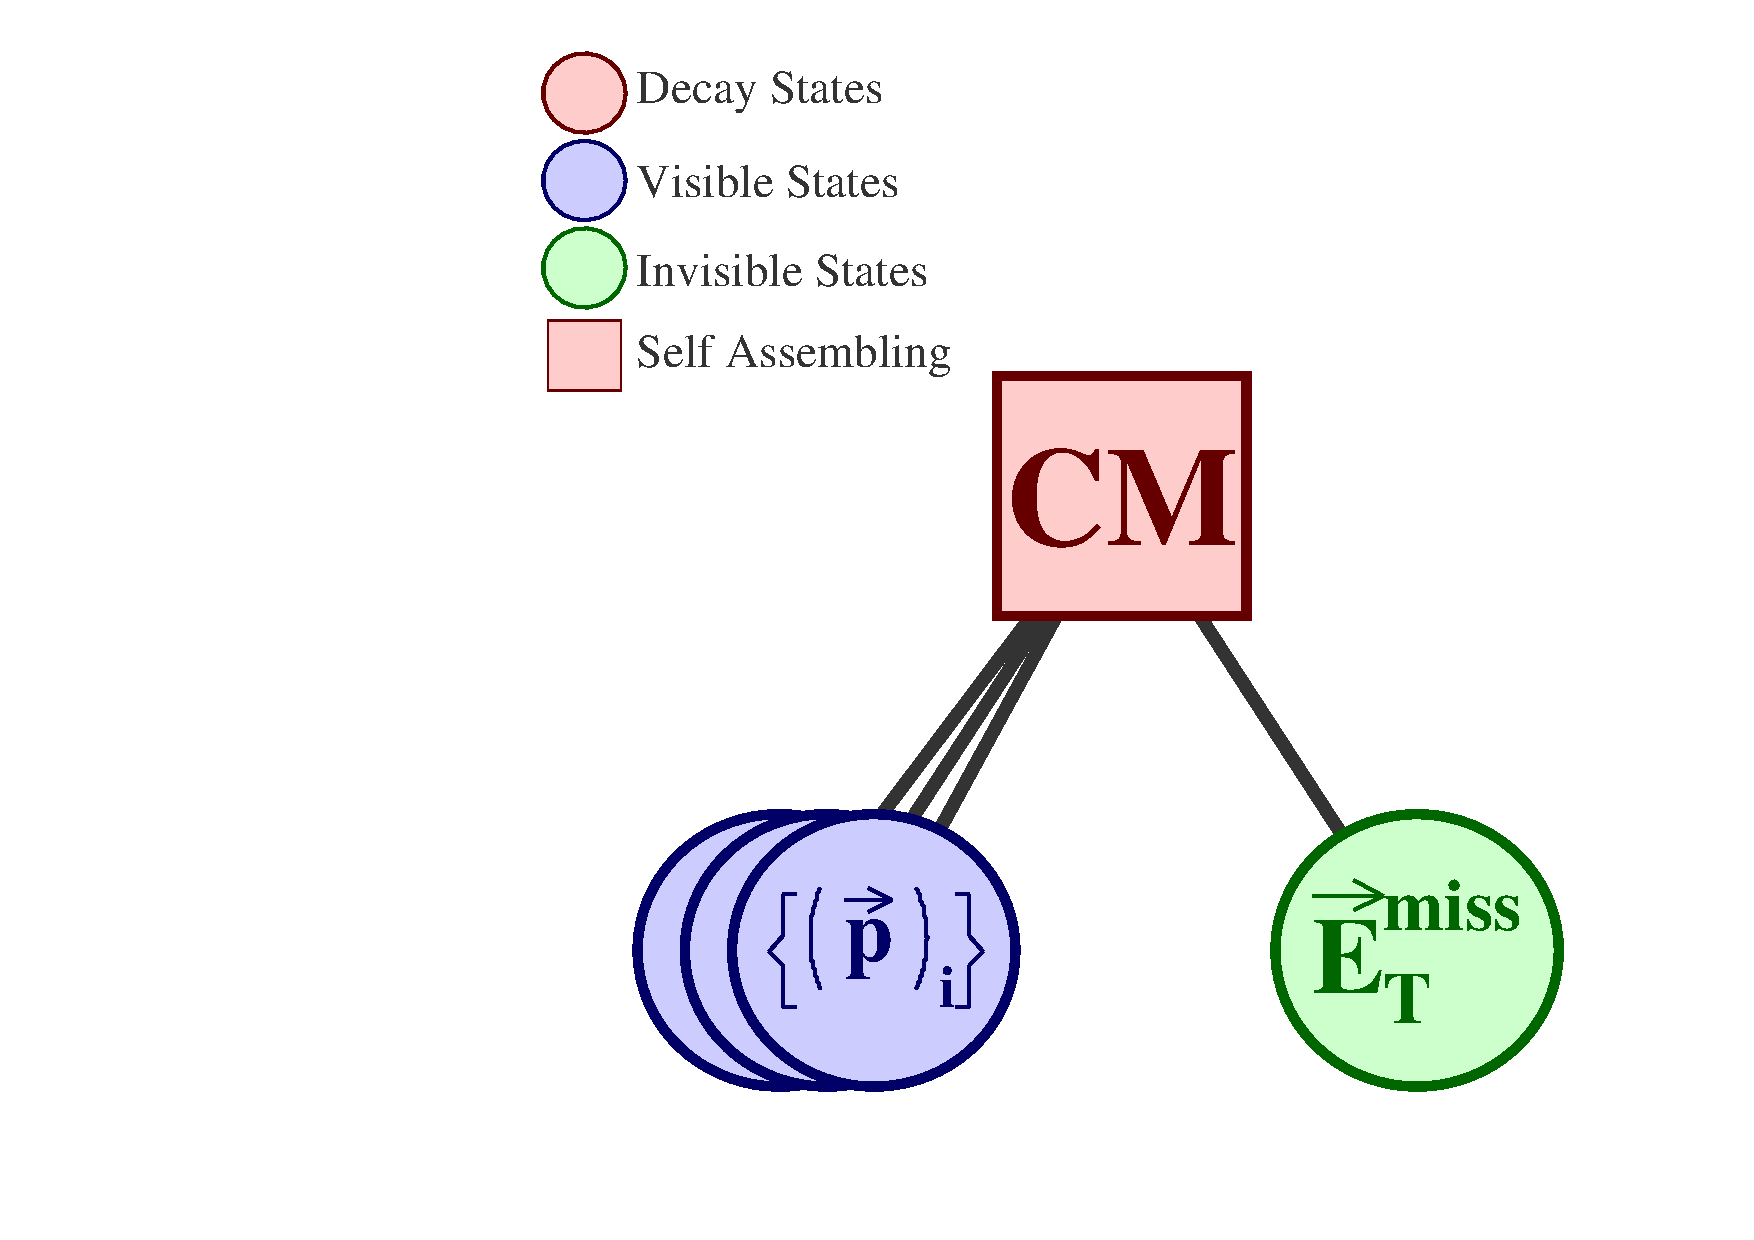
\includegraphics[width=.45\linewidth]{ATLAS-CONF-2016-078_INT/QCD/RJRtree_SelfAssembling}}
\end{figure}
Leaving temporarily the question of ``how'' we apply the jigsaw rules, let us compare these trees to the signal processes of interest.
In particular, we want to compare the Feynman diagrams of \Cref{fig:feynman_signal} with the decay trees of \Cref{fig:decay_trees}.
The decay tree in \Cref{subfig:disquark_decay_tree} corresponds exactly to that expected from squark pair production, and matches closely with the principles of the razor approach.
We first apply a jigsaw rule, indicated by a line, to the kinematics of the objects in the \textit{lab} frame.
This outputs the kinematics of our event in the \textit{parent-parent} (\PP) frame, or in the razor terminology, the CM frame.
That is, the kinematics of this frame are an estimator for the kinematics in the center of mass frame of the CM of pass of the squark pair production system.
We apply another jigsaw, which splits the objects in the \PP frame into two new frames, known as the \Pa and \Pb systems.
These are equivalent to the razor frames, and represent proxy frames where each squark is at rest.
In \Pa (\Pb), the decay is symmetric between the visible \Va (\Vb) objects and the invisible system \Ia (\Ib).
To generate the estimator of the kinematics of the \Va, \Vb, \Ia, and \Ib systems in the \Pa and \Pb systems, we apply another jigsaw rule to split the total \met between \Pa and \Pb.
For the case of squark pair production, this is the expected decay tree, and we stop the recursive calculation at that level.

In the case of gluino pair production, we expect two additional jets, and we can perform an additional boost in each of \Pa and \Pb, to what we call the \Ca and \Cb frames.
The decay tree is shown in \Cref{subfig:digluino_decay_tree}.
In this case we apply a jigsaw at the level of \Pa (\Pb) which separates a single visible object $V_{1a}$ ($V_{2a}$) from the child frame \Ca (\Cb).
This child frame represents the hypothesized squark after the decay $\supe{g} \rightarrow g \supe{q}$, which then decays as in the squark case.

The third decay tree used in this thesis is the \textit{compressed} decay tree.
Compressed refers to signal models which have a small splitting between the mass of the proposed sparticle and the \lsp.
The sparticle decay products in compressed models (i.e. the jets and \met) do not generally have large scale~\cite{Jackson:2016mfb}.
Instead, the strategy is generally to look for a large-scale initial state radiation (ISR) jet which is recoiling off the pair-produced sparticles.
In the case where the LSPs receive no momentum from the sparticle decays, the following approximation holds:
\begin{align}
\met \order -p_T^{\text{ISR}} \times \frac{m_{\lsp} }{m_{\text{sparticle}}}
\end{align}
where $\pt^{\text{ISR}}$ is the transverse momentum associated to the entire ISR system.

RJR offers a natural and straightforward way to exploit this feature in events containing ISR.
One imposes the simple decay tree in \Cref{subfig:compressed_decay_tree} with associated jigsaw rules.
With suitable jigsaw rules, this decay tree ``picks out'' the large \pt ISR jet, recoiling off the \met and additional radiation from the sparticle decays.
This provides a convenient set of variables to understand compressed scenarios.

There is one other decay tree, shown in \Cref{subfig:self_assembling_decay_tree}.
This is special, as it is only used for the purpose of QCD rejection, and does not directly map to a sparticle decay chain.
Due to the large production cross-sections of QCD events, even very rare large jet mismeasurements can lead to significant \met which can enter the signal region.
To reduce these backgrounds, one usually rejects events which contain jets which are ``too close'' by some distance metric to the \met in the event.
Generally, in the past, the distance metric has been defined as simply the angular distance \deltaR.

The \textit{self-assembling tree} can be seen as defining a distance metric which depends on the magnitudes of the \met and jets rather than simply their distance in angular space.
Depending on the exact kinematics, the one or two closest jets are found, and label the \met \textit{siblings}.

In this section, we have seen how one imposes particular decay trees on an event to produce a basis of kinematic variables in the approximated frames relevant to the hypothesized sparticle decay chain.
This explains why we call this procedure ``recursive'': the procedure can be iterated through as many steps of a decay tree as necessary, and each application of a jigsaw rule is dependent on the variables produced in the last step.
The question is: \textit{what are these jigsaw rules?}.

\subsection{Jigsaw Rules}

Jigsaw rules are the fundamental step that allow the recursive definitions of the variables of interest.
The rules we imposed must fully defined kinematic variables at each step in a decay tree.
The only possible solution to fully define the event kinematics in terms of the frames of the hypothesized decays is the imposition of external constraints to eliminate additional degrees of freedom.
In principle, these need not have any particular physical motivation.
Instead, the jigsaw rules are a way to resolve the mathematical ambiguities to fully reconstruct the full decay chain kinematics.
However, most practical jigsaw rules also have some reasonable physical motivation, which we will also elucidate.

In the original razor point of view, some jigsaw rules can be seen as the definitions of the boosts which relate the different frames of interest, while other rules allow one to combine multiple objects and place them into a particular hemisphere (previously megajet).
These are the two forms of jigsaw rules: combinatoric and kinematic.
As we have stressed before, the jigsaw rules are a \textit{choice}: as long as a particular jigsaw rule allows the definition of variables at each step in a decay tree, it is ``as valid'' as any other rule.

Practically speaking, we use only a small subset of possible jigsaw rules.
The combinatoric jigsaw rule has already been introduced as megajet construction above.
The minimization of
\begin{align}
m_{J_1}^2 + m_{J_2}^2.
\end{align}
is a jigsaw rule to deal with the combinatoric ambiguity implicit in which jets go in which hemisphere.
This is the jigsaw rule used in the decay trees when going from one frame to two frames such as \PP $\rightarrow$ \Pa,\Pb.

We will use three other jigsaw rules, which are all kinematic jigsaw rules.
One has already been used in the razor technique.
The minimization of $\beta_L$ will be used as the jigsaw rule in the first step of each decay tree: the lab frame to the \PP/CM frame.
This is equivalent to the imposition of longitudinal boost invariance, as we expect on average $p_{z,\text{\PP,CM}} = 0$.
One defines a unique longitudinal boost by imposition of this external constraint.

The final two jigsaw rules used in this thesis was not used in the razor technique.
We describe them here.

The first kinematic ambiguity is the total mass of the invisible system $M_I$.
We guess this to be:
\begin{align}
M_I^2 = M_V^2 - 4 M_{\Va} M_{\Vb}.
\end{align}
As we stated above, there is no need to ``justify'' the jigsaw rules, as they are in some ways a mathematical trick to fully resolve the event kinematics.
The symmetry of the production mechanism, where we have two decay products $V_i$ and $I_i$ produced from the decay of the same heavy sparticle, is explicit with this jigsaw choice.

The final jigsaw rule is used to resolve the ``amount'' of \met that ``belongs'' to each hemisphere, and therefore how to impose the transverse boost onto each of i.e. \Pa and \Pb from \PP.
Equivalently, it can be seen as the resolution of the kinematics of the \Ia and \Ib objects in the squark and gluino pair production decay trees.
Recall that at this point, we have already approximated the boost of the \PP frame.
The choice we use is to minimize the masses $\Pa$ and $\Pb$, while simultaneously constraining $\Pa = \Pb$.
As is the case in the last step, there is a straightforward physical interpretation of this choice.
In the signal models we are considering, \Pa and \Pb are the estimated frames of the squark or gluino pair-produced as a heavy resonance.
We then of course expect $M_{\Pa} = M_{\Pb}$.

The imposition of the decay trees, with ambiguities resolved through the jigsaw rules, give a full set of boosts relating the frames of each decay tree.
In each frame, we have estimates for the frame mass and decay angles, which can be used in searches for new physics.
In the next section, we describe the variables that are used in this thesis in more details.

\section{Variables used in the search for zero lepton SUSY}
\label{sec:rjr_hadronic}

We describe here the variables used in the RJR search described in~\cite{ATLAS-CONF-2016-078}.
These were reconstructed using the RJR algorithm as just described, using the RestFrames packages~\cite{RestFrames}.
In these frames, the momenta of all objects placed into that branch of the decay tree are available (after application of the approximated boost), and in principle we can calculate any variable of interest such as invariant masses or the angles between these objects.
The truly useful set of variables are highly dependent on the signal process, and we leave their discussion to the subsequent sections.
It is useful to understand the philosophy employed in the construction of these variables.

In general, we can split variables useful for searches for new physics into two categories: \textit{scaleful} and \textit{scaleless} variables.
In this search, we will use a set of scaleful variables called the $H$ variables.
The scaleless variables will consists of ratios and angles.
In general, we want restrict the number of scaleful cuts we apply, for two reasons.
Different scaleful variables are often highly correlated, and this of course limits the utility of additional cuts.
Additionally, selections based on many scaleful variables often overoptimize for particular signal model of interest, especially as related to the mass difference chosen between the sparticle and the LSP.
To avoid this, each decay tree will only use two scale variables, one which quantifies the overall mass scale of the event, and another which acts as a measure of the event balance.

\subsubsection{Squark and gluino variables}

Taking our general philosophy to a particular case, we here describe the variables used by the squark and gluino searches.
We have a suite of scale variables which we will call the $H$ variables, and a suite of angles and ratios.

As we have described above, the RJR algorithm gives us access to the masses of each frame of interest.
It may seem natural that these variables would be the most useful for discrimination of the signal from background processes.
However, these masses, such as the invariant mass of the \PP system $M_{\PP}$, can be significantly affected by the additional jets in the events.
In backgrounds with significant jet activity such as \zjets and \wjets events, these masses can have large values which complicate discrimination from the signal processes.
Instead, we use the $H$ variables, as they show resilience to this effect, and provide stronger discrimination from the SM backgrounds.
They take their name from the commonly used variable \HT, which is the scalar sum of the visible momentum.
From the RJR technique, we can evaluate these variables in the non-lab frame and include longitudinal information.
They are also constructed with \textit{aggregate} momenta using a similar mass minimization procedure as we have already described.

We label these variables as $H_{n,m}^F$.
They are evaluated in the frame $F$, where $F \epsilon \{$lab, \PP, \Pa, \Pb$\}$.
When the discussion applies to both \Pa and \Pb, we will write $P_i$.
The subscripts $n$ and $m$ denote the number of visible and invisible vectors considered, respectively.
When there are more vectors available than $n$ or $m$, we add up vectors using the hemisphere (megajet) jigsaw rule until there are $n$ ($m$) objects\footnotemark.
\footnotetext{Recall that these vectors are constructed by the imposition of the decay tree with the relevant jigsaw rules.}
In the opposite case, where $n$ or $m$ is greater than the number of available objects, one simply considers the available objects.
The \HFnm{F}{n}{m} variables are then defined as
\begin{align}
\HFnm{F}{n}{m} = \sum_i^n | \vec{p_{\text{vis},i}}^F | + \sum_j^m | \vec{p_{\text{inv},i}}^F |.
\end{align}
It may not be clear that these variables encode independent information.
Fundamentally, this is just an expression of the triangle inequality $\sum |\vec{p}| \geq |\sum \vec{p}|$.
One can also define purely transverse of these variables, which we will denote \HTFnm{F}{n}{m}.
Including this view, it is easy to see how the $H$ variables are extensions of the normal \HT variables, as
\begin{align}
\HT = \HTFnm{\text{lab}}{\infty}{0}.
\end{align}

Although the $H$ variables are interesting in their own right, the true power of the RJR technique comes from the construction of scaleless variables.
The scaleless ratios and angles are in fact measured in the ``right'' frame, where right here means an approximation of the correct frame.
This provides a less correlated set of variables than those measured in the lab frame, due to the corrections to the disparticle or sparticle system boosts from the RJR technique.

To search for noncompressed squark pair production, we use the following set of RJR variables:
\begin{itemize}
\item \HFnm {\PP}{1}{1} - scale variable useful for discrimination against QCD backgrounds and used in a similar way to \met
\item \HTFnm{\PP}{2}{1} - scale variable providing information on the overall mass scale of the event for squark pair production.  We will often call this the \textit{full} scale variable.
\item $\HTFnm{\PP}{1}{1}/\HFnm{\PP}{2}{1} $ - ratio used to prevent imbalanced events where the scale variable is dominated by one high \pT jet or high \met
\item \pzlabratioTwo - ratio which prevents significant boosts in the $z-$direction.  \pzlab is a measure of the total boost of the \PP system from the lab frame
\item \ptjTworatio - ratio to force the second leading jet in the \PP frame to carry a significant portion of the total scalar sum of the total momenta in that frame.  This requirement is another balance requirement, on the total \pT of that second jet in the \PP frame.
\end{itemize}
First, we note that there is an implicit requirement that each hemisphere has at least one jet (to even reconstruct the \Pa and \Pb frames), thus we implicitly require two or more jets, as we expect for squark pair production.
The other important thing to note is that all of the ratios use the full scale variable as the denominator.
This is sensible, as we expect all of these effects to be scaled with the full scale variable \HTFnm {\PP}{2}{1}.
We will see a similar behavior for the gluino regions, with a new full scale variable.

To search for noncompressed gluino pair production, we use the following set of RJR variables:
Due to the increased complexity of the event topology with four jets, there are additional handles we can exploit:
\begin{itemize}
\item \HFnm {\PP}{1}{1} - same as squark pair production variable
\item \HTFnm{\PP}{4}{1} - scale variable providing information on the overall mass scale of the event for gluino pair production.  As before, we often call this the \textit{full} scale variable.  Since this variable allows the jets to be separated in the \PP frame, it is more appropriate for gluino pair production.
\item $\HTFnm{\PP}{1}{1}/\HFnm{\PP}{4}{1} $ - ratio used to prevent imbalanced events where the scale variable is dominated by one high \pT jet or high \met
\item $\HTFnm{\PP}{4}{1}/\HFnm{\PP}{4}{1} $ - ratio used to measure the fraction of the total scalar sum of the momentum in the transverse plane.  Decay products from gluino pair production are expected to be fairly central
\item \pzlabratioFour - ratio to used to prevent significant boosts in the $z-$direction
\item \minjTwoGuy - ratio to require the second leading jet in \textit{both} squark-like hemispheres \Ca and \Cb to contain a significant portion of \textit{that frame's} momenta.  This is similar to the \ptjTworatio squark decay tree discriminator, but applied to both hemispheres \Ca and \Cb.
\item \maxjTwoGuy - ratio requiring one jet in each of the $P_i$ not encompass too much of the total momentum available in that frame.  This ratio is generally a very loose cut.
\end{itemize}

\subsubsection{Compressed variables}

As we saw above, the decay tree imposed for compressed spectra is simpler.
We do not attempt to fully reconstruct the details of the system recoiling off the ISR system, but use a straightforward set of variables in this case.
One additional simplification is that all variables are force to be transverse in this case, by simply excluding the $\eta/z$ information of the objects as inputs to the RJR reconstruction.
We still use the philosophy of limiting our scaleful variables to just two.
The compressed scenario uses the following set of RJR variables:
\begin{itemize}
\item \ptisr - scale variable that is the magnitude of the total transverse momenta of all jets associated to the ISR system, as evaluated in the CM frame
\item $\risr \equiv \vec{p_I^{\text{CM}}} \cdot \hat{p_{T,S}^{\text{CM}}} / p_{T,S}^{\text{CM}} $  - this ratio is our measurement for the ratio of the LSP mass to the compressed sparticle mass. In compressed cases, this should be large, as this estimates the amount of the total CM $\rightarrow S$ boost carried by the invisible system.
\item \MTS - the transverse mass of the S system
\item \NVjet - the number of jets associated to the visible system V
\item \dphiISR - the opening angle between the ISR system and the invisible system measured in the lab frame.  As the invisible system is expected to carry much of the total $S$ system momentum, this should be large, as we expect the ISR system to recoil directly opposite the $I$ system.
\end{itemize}

\subsubsection{Anti-QCD variables}

For the self-assembling tree, we construct two variables, which we combine to form a single variable which rejects QCD events.
In this case, we use the mass minimization jigsaw, with a fully transverse version of the event (i.e. we set all jet $z/\eta$ components to 0).
This jigsaw defines the distance metric, and provides us with one or two jets known as the \met siblings.
We define \psib as the sum of these jets, and define the following quantities.

We calculate a ratio observable which examines the relative magnitude of the sibling vector \psib and \met, and an angle relating \psib and \met:
\begin{align}
R( \psib, \met )          & \equiv \frac{\psib \cdot \methat}{ \psib \cdot \methat + |\metvec|} \\
\cos{\theta(\psib, \met)} & \equiv \frac{ (\psib + \metvec) \cdot \hat{p^{\text{sib+miss}_{sib}}}}{|\psib| + \met}
\end{align}
These observables are highly correlated, but taking the following fractional difference provides strong discrimination between SUSY signal and QCD background events:
\begin{align}
\Delta_{\mathrm{QCD}} \equiv \frac{1 + \cos{\theta(\psib, \met)} - 2 R(\psib, \met) }{1 + \cos{\theta(\psib, \met)} + 2 R(\psib, \met) }.
\end{align}
We will use this variable in the next chapter.

\section{Conclusions}

The RJR suite of variables will provide sensitivity to a wide variety of squark and gluino production scenarios.
We will see in the next chapter that this set of variables described above provide strong sensitivity to a wide range of simplified models of squark and gluino pair production, by use of a variety of signal selections, in the next chapter.
We note however, that this set of variables is not unique, and the RJR technique can be used for a large variety of final states.
The search presented here is the first to use RJR, but a different suite of variables could be used for other decay modes, and it will be exciting to see how the technique can be exploited in future searches.